\chapter{Approach and Methodology}
\label{cha:research_method}

This chapter describes the steps we took to answer the research question \textit{how can a location-based freecycling service reduce the social isolation of forced migrants?}, which we introduced and motivated in chapter~\ref{cha:introduction} and grounded in existing research in chapter~\ref{cha:background}.

We used human-centered design principles to structure our methodology due to its suitability when designing services for forced migrants, as explained in section~\ref{sec:hcd}. We applied the human-centered design process in three phases, each correlating to one of our angles of approach. In the first phase we performed a needs assessment study, carrying out interviews and extracting context and user requirements from the data. In the second phase we developed a prototype location-based freecycling service based on the needs identified. In phase three we carried out a user study to evaluate the prototype design.

Each phase answered our research question in a different way and produced a unique contribution. Phase one answered the question theoretically and produced a list of needs and user requirements. Phase two answered the question technologically and produced a working prototype demonstrating the feasibility of the designs. Phase three answered the question in the field and resulted in validation of the usability of the designs and a preliminary assessment of the usefulness of location-based services for the reduction of forced migrant isolation.

\begin{figure}[ht]
  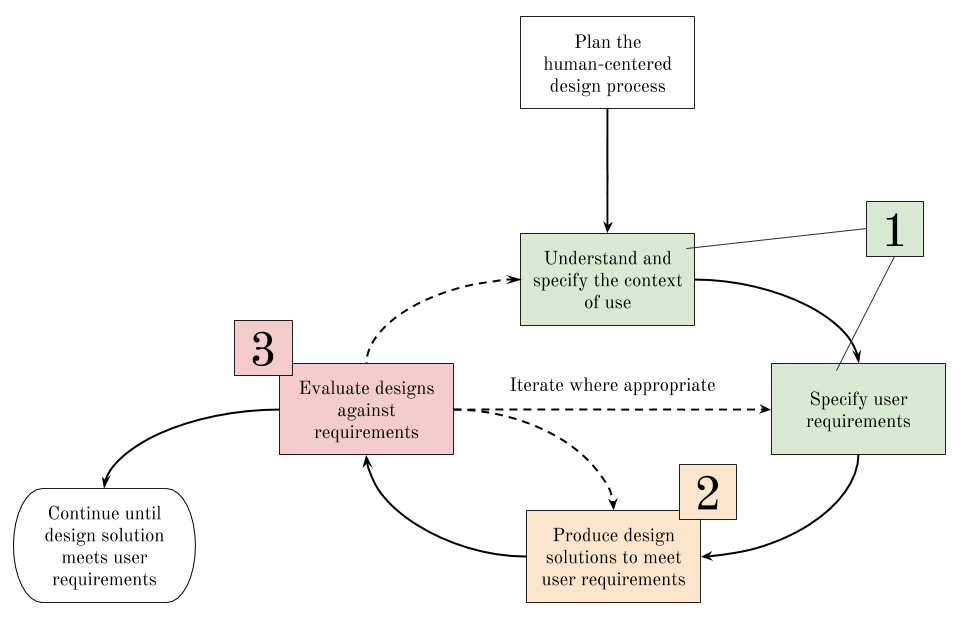
\includegraphics[width=\textwidth]{images/human_centered_design_flowchart_divided.png}
  \caption{The human-centered design process divided into three phases}
  \label{fig:hcd_divided}
\end{figure}

The three parts took different forms. First we ran a user study to assess the needs of our user groups and develop user requirements for a hypothetical system. Then we developed a prototype designed to meet those needs, making the hypothetical real. Finally we ran another user study to evaluate the prototype. The following three chapters describe the needs assessment, prototype development, and prototype evaluation in full detail.

While valuable for its simplicity, the presentation of our methodology as three steps conceals the iterative nature of human-centered design. In this work we did not follow the three steps linearly but rather continually moved among them. Neither are we recommending that others follow a stricter step-by-step process. Continual adjustment of needs assessments, implementations, and evaluations is necessary to address the continually evolving context of forced migrant resettlement.

Per the ISO definition, human-centered design consists of 5 steps, 4 of which may need repeating several times. They are: 1) plan the human-centered design process, 2) understand and specify the context of use, 3) specify user requirements, 4) produce design solutions to meet user requirements, and 5) evaluate designs against requirements. Figure~\ref{fig:hcd_divided} shows how these steps proceed in a cyclical manner until a satisfactory solution is achieved. Each of these steps yielded distinct results in this study. Following is a step-by-step overview of how we applied the human-centered design process to address the research question of this thesis. The exact methodology and results of the process are described in detail in the subsequent three chapters.

\textit{1. Planning the human-centered design process.} Before beginning this work, we wrote up a detailed plan and assessed the feasibility of the various steps. We outlined roughly when and how each of the four remaining steps would be achieved, leaving room for iteration. We identified three user groups to be at the center of the design process. We verified the availability of potential participants from the three user groups to do context interviews. We also reviewed existing literature about technology for forced migrants and freecycling systems in order to build our understanding of the context of use. The results of this process are discussed in chapter~\ref{cha:background}.

In this initial phase, we also planned out which technologies we would use as a starting point for the design solutions, and we sketched out a plan for evaluating these designs at the end. We met personally with local experts from forced migrant and freecycling communities to glean their recommendations about how to implement our design process. Young forced migrants expressed interest in new technology and committed to help with the design process and find others to participate too. Freecycling system moderators told us how to get in touch with their users, shared common freecycling challenges and provided assurance that the design of a new freecycling platform for forced migrants would be supported by their communities.

\textit{2. Understanding and specifying the context of use.} In this study, understanding the context of use meant investigating why and how forced migrants currently make social contact in Münster. Additionally, it meant learning about existing freecycling systems in the city. We used context interviews to achieve both of these tasks. The details of this process are described in chapter~\ref{cha:needs}.

\textit{3. Specifying user requirements.} In order to identify key user requirements for a location-based freecycling service, we began by extracting implied needs from the context interviews. These in turn were translated into user requirements. See chapter~\ref{cha:needs} for the results of this process.

\textit{4. Producing design solutions to meet user requirements.} The second phase of the study was designing and implementing a prototype app. We decided to make a cross-platform mobile app based on the location-based service app engine called LBS Engine \cite{einfeldt_lbs_2018}. See chapter~\ref{cha:prototype} for a full description of the implementation process and results.

\textit{5. Evaluating the designs against the requirements.} The designs were evaluated in an iterative fashion, first by having individuals test the prototype in my presence, then by running a pilot deployment to a small group of fellow students, and finally by deploying the prototype app to a larger group for a two-week trial period. During the trial, we collected data from users as we had planned. See chapter~\ref{cha:evaluation} for full details and a discussion of the results of the evaluation.